\documentclass{article}
\usepackage{tikz, comment}
\usepackage{pifont}
\usepackage{fontspec, pgfplots}
\usetikzlibrary{arrows, decorations.markings, decorations.pathreplacing}
\begin{comment}
:Title: Not defined yet
:Tags: absolute value rules;properties of equality, equation rules;set;equivalence properties of equality;trichotomy
:Prob: 0.678;0.6228;0.6093;0.5839;0.5728
:Author: Prof.Hu Ji-shan, HKUST
:Slug: No name yet

Description Here.........
\end{comment}
\begin{document}\centering 

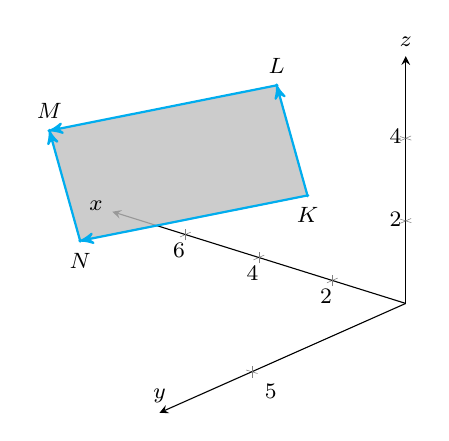
\begin{tikzpicture}[font=\footnotesize]
\pgfplotsset{compat=1.8}
\begin{axis}
[axis lines = center, view={220}{30}, scale=1., %ticks=none, 
axis background, xlabel = {$x$}, ylabel ={$y$}, zlabel ={$z$}, domain =0:1, y domain =0:1,
xmin =0,
xmax =7.99,
ymin =0,
ymax =8,
zmin =0, 
zmax =5.99,
samples =10, samples y =40, z buffer =sort,
every axis x label/.style={
    at={(ticklabel* cs:1)},
    anchor= east, yshift =2
},
every axis y label/.style={
    at={(ticklabel* cs:1)},
    anchor= south,
},
every axis z label/.style={
    at={(ticklabel* cs:1)},
    anchor= south
}]

\addplot3[surf, lightgray, mesh/cols=2, opacity=0.8] coordinates
        {(1,2,3) (1,3,6) (3,7,3) (3,8,6) };
          
\addplot3[cyan, thick, ->, >=stealth'] coordinates
        {(1,2,3) (1,3,6)};
\node[xshift=0, yshift=0, label={-90:{$K$}}, circle,fill=cyan,inner sep=0.5pt] at (axis cs:1,2,3) {};

\addplot3[cyan, thick, ->, >=stealth'] coordinates
        {(1,3,6) (3,8,6)};        
\node[xshift=0, yshift=0, label={90:{$L$}}, circle,fill=cyan,inner sep=0.5pt] at (axis cs:1,3,6) {};

\addplot3[cyan, thick, ->, >=stealth'] coordinates
        {(3,8,6) (3,7,3)};
\node[xshift=0, yshift=0, label={90:{$M$}}, circle,fill=cyan,inner sep=0.5pt] at (axis cs:3,8,6) {};

\addplot3[cyan, thick, ->, >=stealth'] coordinates
        {(3,7,3) (1,2,3)};  
\node[xshift=0, yshift=0, label={-90:{$N$}}, circle,fill=cyan,inner sep=0.5pt] at (axis cs:3,7,3) {};

\end{axis}

\end{tikzpicture}
\end{document}